%% LyX 2.2.2 created this file.  For more info, see http://www.lyx.org/.
%% Do not edit unless you really know what you are doing.
\documentclass[11pt,english]{beamer}
\usepackage{enumerate}

\usepackage{mathptmx}
\usepackage[T1]{fontenc}
\usepackage[utf8]{inputenc}
\setlength{\parskip}{\smallskipamount}
\setlength{\parindent}{0pt}
\usepackage{url}
\usepackage[authoryear]{natbib}
\usefonttheme[onlymath]{serif} % para las fuentes de las ecuaciones
\makeatletter
\usepackage{amsmath,amssymb,amsthm}
\usepackage{graphicx}
\usepackage{xcolor} % para colorear textos con \textcolor o \color
\usepackage{hyperref}
\usepackage{times}
\usepackage{array}
\usepackage{multicol}
\usepackage{longtable}
\usepackage{float} % para usar comando [H] en tablas y gr\'aficas
\usepackage{xcolor}% para modificar el color de la presentacion y del texto
\usepackage{colortbl} % para tablas de Kable
\usepackage{booktabs} % Para toprule: To thicken table lines 
\usepackage[nogin]{Sweave} % elimina el tamaño por default de las figuras de sweave
\usepackage{natbib}
\bibliographystyle{agsm}
% \usepackage[inline]{enumitem} % para enumerar dentro de un paragrafo
\usepackage{rotating} % para rotar nombres de columnas

\usepackage{fancyvrb} % Ensure this line is in your preamble
\usepackage{graphicx}
\usepackage{subcaption}

\usepackage{listings} % esta y la siguiente para resolver el problema del FancyVerb 
\lstset{basicstyle=\ttfamily} % esta tambien para lo del FancyVerb 



%%%%%%%%%%%%%%%%%%%%%%%%%%%%%% LyX specific LaTeX commands.
\providecommand{\LyX}{L\kern-.1667em\lower.25em\hbox{Y}\kern-.125emX\@}

%%%%%%%%%%%%%%%%%%%%%%%%%%%%%% Textclass specific LaTeX commands.
 % this default might be overridden by plain title style
 \newcommand\makebeamertitle{\frame{\maketitle}}%
 % (ERT) argument for the TOC
 \AtBeginDocument{%
   \let\origtableofcontents=\tableofcontents
   \def\tableofcontents{\@ifnextchar[{\origtableofcontents}{\gobbletableofcontents}}
   \def\gobbletableofcontents#1{\origtableofcontents}
 }
\newcommand{\code}[1]{\texttt{#1}}

%%%%%%%%%%%%%%%%%%%%%%%%%%%%%% User specified LaTeX commands.
\usetheme{Warsaw}
% or ...

\setbeamercovered{transparent}
% or whatever (possibly just delete it)

\usepackage[T1]{fontenc}

\makeatother

\usepackage{babel}
\usepackage{listings}
\renewcommand{\lstlistingname}{\inputencoding{latin9}Listing}

\begin{document}
\Sconcordance{concordance:6_ACM-2025-I.tex:6_ACM-2025-I.Rnw:1 52 1 1 4 50 1 5 4 1 1 1 %
4 1 5 3 4 309 1 1 18 3 1 1 7 23 0 1 2 7 1 2 2 7 1 1 6 33 0 1 2 19 1 1 3 %
1 2 11 1 1 3 1 2 5 1 1 16 5 1 1 3 1 2 7 1 1 3 1 2 26 1}



\title{Análisis de Correspondencias Múltiples (ACM)}

\subtitle{Introducción}

\author{Jimmy A Corzo S\inst{1} \inst{2}}

\institute[Profesor Titular]{\inst{1}Profesor Titular\\
Departamento de Estadística\and \inst{2}Facultad de ciencias\\
Universidad Nacional de colombia}

\date[2023]{Métodos multivariados aplicados \LyX{} cap 3}

\makebeamertitle

%\pgfdeclareimage[height=0.5cm]{institution-logo}{institution-logo-filename}

%\logo{\pgfuseimage{institution-logo}}

\AtBeginSubsection[]{

  \frame<beamer>{ 

    \frametitle{Outline}   

    \tableofcontents[currentsection,currentsubsection] 

  }

}













%\beamerdefaultoverlayspecification{<+->}
\begin{frame}
\tableofcontents{}
\end{frame}

\section{Descripción del método}
\begin{frame}{Introducción}
El ACM es una generalización natural del ACS a más de dos variables cualitativas. El método se realiza sobre una \textbf{Tabla de Tablas de contingencia} llamada también tabla de Burt, que es una tabla formada por bloques, cada uno de los cuales es una tabla de frecuencias entre un par de variables\footnote{La equivalencia entre un ACM entre dos preguntas y un ACS se puede consultar en \cite{lebart1984}, secc IV.2, pág 84.}. 
\end{frame}
% 
\begin{frame}{Introducción}
El contexto a que se refiere el ACM  asume que $n$ individuos contestan un instrumento de $Q$ preguntas, cada una de las cuales tiene $p_{_q}$ opciones o modalidades de respuesta. Las respuestas para a la pregunta $q$ se encuentran almacenadas en una matriz disyuntiva $Z_q$ de dimensiones $n\times p_q$ cuyos elementos son:
$$
Z_q=\left\lbrace z_{q(ik)} \right\rbrace, i=1,\ldots n, \quad k=1,\ldots p_{_q} \quad q=1,\ldots Q,
$$
donde
\footnotesize
\begin{align*}
	z_{q(ik)}=
\begin{cases}
  1 & \text{si el $i$-ésimo individuo seleccionó la opción $k$ de la pregunta $q$} \\
  0 & \text{si no}
\end{cases}
\end{align*}
\end{frame}
% 
\begin{frame}{Ejemplo}
Por ejemplo, si la pregunta $q$ con $p_{q} = 3$ opciones de respuesta ($o1,\, o2 \, y \, o3$), la tabla disyuntiva $z_{q}$ tiene la forma:

$$ 
 \begin{array}{c|ccc|c}
ind & p_q\, o1 & p_q \, o2  & p_q \, o3 & Suma\\
\hline
1   & 1 & 0 & 0 & 1\\
2   & 0 & 0 & 1 & 1\\
\vdots   & \vdots & \vdots & \vdots & \vdots\\
j   & 1 & 0 & 0 & 1\\
\vdots   & \vdots & \vdots & \vdots & \vdots\\
n   & 0 & 1 & 0 & 1\\
 \end{array}
$$
\end{frame}
% 
\begin{frame}{Descripción y tabla de datos}
Sea $p=\sum_{q=1}^{Q}p_q$ el número total de modalidades de respuesta en todo el instrumento. Ahora se arreglan las respuestas a todas las preguntas de la encuesta en una \textbf{matriz disyuntiva completa} de dimensiones $n \times p$:
\[ Z= \left[ Z_1,Z_2,\cdots,Z_{_Q} \right] \]


\end{frame}
% 
\begin{frame}
La estructura de la tabla correspondiente a las matriz disyuntiva completa $Z$ con los totales por fila que producen el número de preguntas y por columna que producen el número de individuos que contestaron cada opción de respuesta es la siguiente:
$$ 
 \begin{array}{c|ccc|cc|c|ccc|c|}
i & p_1\,o1  &  p_1\, o2 &  p_1\, o3 & p_2\,o1 & p_2\,o2 & \ldots & p_q\,o1 & p_q\, o2 & p_q\, o3  & z_{i.} \\
\hline
1   & 1 & 0 & 0                        & 1       &   0      & \ldots & 1       & 0        & 0        & Q\\
2   & 0 & 0 & 1                        & 0       &   1      & \ldots & 1       & 0        & 0        & Q\\
\vdots   & \vdots & \vdots & \vdots    & \vdots  & \vdots   & \vdots &  \vdots &   \vdots &  \vdots  &\\
n   & 0 & 1 & 0                        & 1       &   0      & \ldots & 0       & 1        & 0        & Q\\
% & & & & & & & & &\\
\hline
& z_{1(\cdot 1)} & z_{1(\cdot 2)} & z_{1(\cdot 3)} & z_{2(\cdot 1)} & z_{2(\cdot 2)} & \ldots & z_{q(\cdot 1)} & z_{q(\cdot 2)} &  z_{q(\cdot 3)} & nQ
 \end{array}
$$
\end{frame}
% 
\begin{frame}{Tabla disyuntiva completa}
En la tabla disyuntiva completa se observa que 
\begin{gather}
\text{la suma por filas produce el \# de preguntas:} \quad z_{i.}=Q =\sum_{j=1}^p z_{ij}\hfill \notag \\
\text{la suma por columnas produce el \# de individuos que contestaron}\hfill \notag \\
\text{la modalidad $j$ de pregunta $q$:} \quad z_{q(.j)}=\sum_{i=1}^n z_{q(ij)}\hfill \notag
\end{gather}
\end{frame}
% 
\begin{frame}{\textcolor{yellow}{Paso de tabla disyuntiva completa a tabla de codigos}}
\scriptsize
\begin{table}[htbp]
  \centering
  \caption{Paso de tabla disyuntiva completa a tabla en códigos}
    \begin{tabular}{c|c|c|c|c|c|c|c|c|c|r|c|c|c|}
    \multicolumn{1}{c}{} & \multicolumn{9}{c}{Tabla disyuntiva completa}                         & \multicolumn{1}{r}{} & \multicolumn{3}{c}{Tabla en códigos} \\
\cmidrule{2-10}\cmidrule{12-14}    ind   & \multicolumn{4}{c|}{$p_1$} & \multicolumn{2}{c|}{$p_2$} & \multicolumn{3}{c|}{$p_3$} &       & $p_1$ & $p_2$ & $p_3$ \\
          & $o_1$ & $o_2$ & $o_3$ & $o_4$ & $o_1$ & $o_2$ & $o_1$ & $o_2$ & $o_3$ &       &       &       &  \\
\cmidrule{1-10}\cmidrule{12-14}    1     & 1     & 0     & 0     & 0     & 1     & 0     & 1     & 0     & 0     &       & 1     & 1     & 1 \\
    2     & 0     & 1     & 0     & 0     & 0     & 1     & 0     & 0     & 1     &       & 2     & 2     & 3 \\
    3     & 0     & 0     & 1     & 0     & 0     & 1     & 0     & 1     & 0     &       & 3     & 2     & 2 \\
    4     & 0     & 0     & 0     & 1     & 1     & 0     & 0     & 1     & 0     & \multicolumn{1}{l|}{$\rightarrow$} & 4     & 1     & 2 \\
    5     & 0     & 0     & 1     & 0     & 1     & 0     & 1     & 0     & 0     &       & 3     & 1     & 1 \\
    6     & 0     & 1     & 0     & 0     & 0     & 1     & 0     & 0     & 1     &       & 2     & 2     & 3 \\
    7     & 1     & 0     & 0     & 0     & 0     & 1     & 0     & 1     & 0     &       & 1     & 2     & 2 \\
    8     & 1     & 0     & 0     & 0     & 1     & 0     & 1     & 0     & 0     &       & 1     & 1     & 1 \\
    9     & 0     & 0     & 1     & 0     & 0     & 1     & 0     & 1     & 0     &       & 3     & 2     & 2 \\
    \end{tabular}%
  \label{tab:addlabel}%
\end{table}%
\end{frame}
% 
\begin{frame}{Tabla de Burt}
Esta tabla se obtiene con el producto de la matriz disyuntiva completa:
\begin{align}\label{burt}
  B=Z'Z =  
 \left[ 
 \begin{array}{cccc} 
  Z_1^\prime Z_1 & Z_1^\prime Z_2 & \cdots & Z_1^\prime Z_Q \\
  Z_2^\prime Z_1 & Z_2^\prime Z_2 & \cdots & Z_2^\prime Z_Q \\
  \vdots         & \vdots         & \vdots & \vdots  \\
  Z_Q^\prime Z_1 & Z_Q^\prime Z_2 & \cdots & Z_Q^\prime Z_Q 
 \end{array}
  \right]
\end{align}
\end{frame}
% 
\begin{frame}{Simetría de la tabla de Burt}
Como se observa la tabla de Burt es una matriz simétrica \textbf{por bloques} tales que:
en la diagonal están las tablas de contingencia  de la pregunta $q$:
\begin{align}
	D_q = Z_q^\prime Z_q =
\left[ 	
	\begin{array}{cccc}
	z_{q(\cdot 1)} &   0       & \ldots &       0 \\
	   0      & z_{q(\cdot 2)} & \ldots &       0 \\
	   \vdots & \vdots         & \vdots & \vdots  \\
	   0      &       0        & \ldots & z_{q(\cdot p_q)}    
	\end{array}
\right] , \quad q=1,\ldots,Q
\end{align}
\end{frame}
% 
\begin{frame}
mientras que por encima y debajo de la diagonal se encuentran las tablas de contingencia $Z_q^\prime Z_{q^\prime}$ entre las preguntas $q$ y $q^\prime$ de dimensiónes $p_q \times p_{q^\prime}$ que tienen la siguiente estructura:
\footnotesize
\begin{align}\label{zTz}
Z_q^\prime Z_{q^\prime} = 
\left[
  \begin{array}{cccc}
  z_{q(1,1)}   & z_{q(2,1)} & \cdots & z_{q(n,1)}\\
  z_{q(1,2)}   & z_{q(2,2)} & \cdots & z_{q(n,2)}\\
  \vdots       & \vdots     & \vdots & \vdots\\
  z_{q(1,p_q)} & z_{q(2,p_q)} & \cdots & z_{q(n,p_q)}
  \end{array}
\right]
\left[
  \begin{array}{cccc}
  z_{q^\prime(1,1)} & z_{q^\prime(1,2)} & \cdots & z_{q^\prime(1,p_{q^\prime})}\\
  z_{q^\prime(2,1)} & z_{q^\prime(2,2)} & \cdots & z_{q^\prime(2,p_{q^\prime})}\\
  \vdots            & \vdots            & \vdots & \vdots\\
  z_{q^\prime(n,1)} & z_{q^\prime(n,2)} & \cdots & z_{q^\prime(n,p_{q^\prime})}
  \end{array}
\right]
\end{align}
\end{frame}
% 
\begin{frame}
cuyos elementos tienen la forma genérica:
\begin{align*}
  \left\lbrace  \sum_{i=1}^n z_{q({ij})}z_{q^\prime({ik})} \right\rbrace
\end{align*}
Entonces, como $z_{q({ij})}z_{q^\prime({ik})} = 1$ solamente cuando el individuo $i$ contestó $j$ de la pregunta $q$ y $k$ de la pregunta $q^\prime$ la suma produce el número de individuos que contestaron la opción $j$ de la pregunta $q$ y la opción $k$ de la pregunta $q^\prime$
\end{frame}
% 
\section{Obtención de las componentes}
% 
\begin{frame}{Distancia entre modalidades de las preguntas}
Modalidades $j$ y $j^\prime$
\begin{equation*}
	d(j,j^\prime) = \sum_{i=1}^n n\left(\frac{z_{ij}}{z{.j}}-\frac{z_{ij^\prime}}{z{.j^\prime}} \right)^2,
\end{equation*}
Entonces dos modalidades dos modalidades están cerca si fueron contestadas aproximadamente por los mismos individuos estarán muy cerca, y de lo contrario estarán lejos.
\end{frame}
% 
\begin{frame}{Distancia entre objetos}
individuos $i$ e $i^\prime$ 
\begin{equation*}
	d(i,i^\prime) = \frac1Q \sum_{j=1}^p\frac{n}{z_{.j}} \left( z_{ij} - z_{i^\prime j} \right)^2.
\end{equation*}
Entonces dos individuos están cerca si contestaron aproximadamente las mismas modalidades y estarán lejos si no coiciden mucho en sus respuestas.
\end{frame}

\begin{frame}{\textcolor{yellow}{Obtención de las componentes}}
De manera similar al ACS, el análisis en el ACM se hace sobre las tablas de perfiles fila y columna pero de la matriz disyuntiva completa. 

Por esta razón, dichos perfiles tienen que ser calculados tanto con respecto al número de preguntas $Q$ como respecto a las frecuencias de respuesta de las preguntas. 

Para el ACM se usan entonces los perfiles fila y columna de la tabla disyuntiva completa, se mantiene el criterio de distancia $\chi^2$ y las interpretaciones son las mismas que las del ACS.
\end{frame}
% 
\begin{frame}
Para saber cómo están formadas las componentes y qué es lo que representan se muestra la matriz a la que se calculan los valores y vectores propios:
\begin{equation}\label{SdeACM}
S=\frac{1}{Q}Z'ZD^{-1} = \frac{1}{Q}BD^{-1}
\end{equation}

donde

\begin{align}
	D^{-1} = 
\left[ 	
	\begin{array}{cccc}
	D_1^{-1}   &   0       & \ldots &       0 \\
	   0       & D_2^{-1}  & \ldots &       0 \\
	   \vdots\\
	   0       &           & \ldots & D_Q^{-1}    
	\end{array}
\right]
\end{align}
\end{frame}
% 
\begin{frame}
\begin{align}
	D_q^{-1} = (Z_q^\prime Z_q)^{-1} =
\left[ 	
	\begin{array}{cccc}
	1/z_{q(\cdot 1)} &   0       & \ldots &       0 \\
	   0      & 1/z_{q(\cdot 2)} & \ldots &       0 \\
	   \vdots\\
	   0      &           & \ldots & 1/z_{q(\cdot p_q)}    
	\end{array}
\right] , \quad q=1,\ldots,Q
\end{align}
\end{frame}

\begin{frame}
Entonces como $B$ es una matriz por bloques definidos en (\ref{burt}) a (\ref{zTz}), los elementos de $S$ tienen la forma:
$$
s_{jk} = \frac{1}{Q}\sum_{i=1}^n \frac{z_{q({ij})}z_{q^\prime({ik})}}{z_{q(.k)}}
$$
%  = \frac{1}{Qz_{.k}}\sum_{i=1}^n z_{q({ij})}z_{q^\prime({ik})},
donde cada sumando es la proporción de respuestas simultáneas a la opción $j$ de la pregunta $q$ y la opción $k$ de la pregunta $q^\prime$. 
Y al estar dividida por $Q$, la suma  es la proporción de la proporción de respuestas simultáneas de las modalidades $j$ y $k$ con respecto al total de preguntas. 
\end{frame}
% 
\section{Varianza (inercia) de opciones de respuesta y de las preguntas}
% 
\begin{frame}{ \textcolor{yellow}{Varianza o Inercia}}
\small
En el contexto del ACS y ACM suele asociarse la varianza de las opciones de respuesta con el concepto físico de \textbf{inercia}, debido a qué una mayor varianza implica un grado de dispersión grande de los datos, idea que se puede asociar con la inercia debido a que una varianza grande implica un mayor radio de acción o de influencia tiene la modalidad o la pregunta (ver por ejemplo \cite{lebart2006statistique}):
\end{frame}
% 
\begin{frame}{Inercia}
\tiny
\begin{itemize}
		\item La varianza (inercia) de  una modalidad se define por:
		\textcolor{blue}{
\begin{equation}\label{inerciamod}
I(j)=\frac{1}{Q}\left( 1-\frac{z_{.j}}{n} \right)
\end{equation}
}
Aumenta cuando pocos individuos la contesten ($z_{.j}$ pequeño).
Disminuye con el número de preguntas $Q$.
		\item La varianza (inercia) de una pregunta completa es el acumulado de las varianzas de las modalidades:
\textcolor{red}{		
\[ I(q)=\sum_{j=1}^{p_q}I(j)=\frac{1}{Q}\sum_{j=1}^{p_q}\left( 1-\frac{z_{.j}}{n} \right)=\frac{1}{Q}(p_q-1). \]
}
Solo depende del \# de modalidades y \# de respuestas, se puede fijar indenpendiente de las proporciones de respuesta. \textbf{no es de interés estadístico}. Ventaja: se puedan diseñar instrumentos con varianza conocida de antemano.
		\item La varianza (inercia) total definida como la suma de las varianzas de las preguntas:
		\textcolor{red}{
\[ IT=\sum_qI(q)=\frac{p}{Q}-1 \]
}
es función del \# de modalidades y \# de preguntas y \textbf{no de la relación entre ellas}, razón por la que \textbf{tampoco es de interés estadístico}.
\end{itemize}
\end{frame}
% 
\begin{frame}{Inercia}
\large
\textbf{La conclusión es que la única varianza (inercia) que tiene interés real para la interpretación es la de las modalidades, porque depende del número o proporción de respuestas que tuvo en la encuesta.}:
		\textcolor{blue}{
\begin{equation*}\label{inerciamod}
I(j)=\frac{1}{Q}\left( 1-\frac{z_{.j}}{n} \right)
\end{equation*}
}
\end{frame}
% 
\section{Guías para la interpretación del ACM}
% 
\begin{frame}{Guías para la interpretación}
\footnotesize
\begin{itemize}
    \item Todas las reglas de interpretación del ACS en cuanto a las coordenadas, las contribuciones y los cosenos cuadrados son aplicables directamente al ACM.
    \item La proximidad entre individuos indica semejanzas entre ellos en el sentido de que éstos seleccionaron aproximadamente las mismas opciones de respuesta.
		\item La proximidad entre opciones de respuesta de preguntas diferentes indica asociación entre éstas debido a que son los puntos medios de los individuos que las seleccionaron. Además, por estar próximas también indican que fueron seleccionadas aproximadamente por los mismos individuos, lo cual indica que éstos tienen opiniones parecidas.
		\item La proximidad entre opciones de respuesta de una misma pregunta también indican semejanzas entre los individuos que las contestaron, debido a que por ser de la misma pregunta son excluyentes y por tanto estar próximas indica que los grupos de individuos que las seleccionaron son parecidos.
\end{itemize}
\end{frame}
% 
\section{Encuesta de Cultura Ciudadana (ECC)}
\begin{frame}{Ejemplo}
La ECC incluye entre sus preguntas una referida si se justifica o no desobedecer la ley en ciertas circunstancias  La pregunta consta de 11 enunciados (items) a los cuales el encuestado debe contestar si  o no según opine si justifica o no desobedecer la ley por la razón mencionada. Se incluyó tambien la ciudad y el nivel educativo como variables suplementarias.
\end{frame}
% 
\begin{frame}{Ejemplo}
\begin{center}
\begin{figure}[H]
\centering
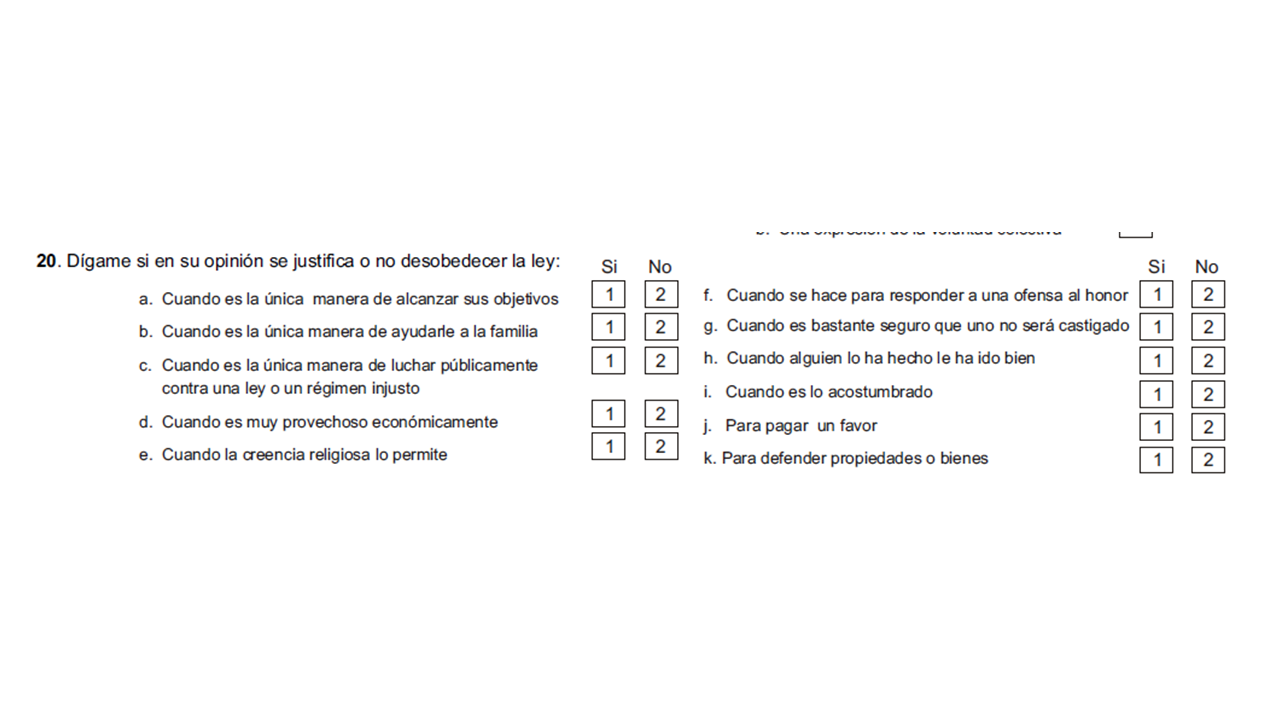
\includegraphics[width=1.1\textwidth]{Justificaciones obdiencia de la ley}
\end{figure}
\label{fig:JustObedecerLey}
\end{center}
\end{frame}
% 
\begin{frame}
En la tabla de valores propios \ref{tab:Vp1ACM} visualizada en la gráfica \ref{fig:Vrspropios}, se observa que el primer valor propio es casi 3.5 veces el segundo, mientras que segundo es un poco más de 1.3 veces el tercero. De ahí en adelante, las variaciones son más pequeñas y por tanto resulta difícil escoger el número de componentes a interpretar. Para este ejemplo se escogen para el análisis las primeras tres compnentes que acumulan casi el  57\% de la varianza.
\end{frame}
% 
% \begin{frame}[fragile]
% \scriptsize
% \end{frame}

% 
\begin{frame}[fragile]
\footnotesize
\begin{table}[!h]
\centering
\caption{\label{tab:vp}Valores propios}
\centering
\resizebox{\ifdim\width>\linewidth\linewidth\else\width\fi}{!}{
\begin{tabular}[t]{lrrr}
\toprule
  & eigenvalue & percentage of variance & cumulative percentage of variance\\
\midrule
\cellcolor{gray!10}{dim 1} & \cellcolor{gray!10}{0.38} & \cellcolor{gray!10}{37.69} & \cellcolor{gray!10}{37.69}\\
dim 2 & 0.11 & 10.81 & 48.50\\
\cellcolor{gray!10}{dim 3} & \cellcolor{gray!10}{0.08} & \cellcolor{gray!10}{8.04} & \cellcolor{gray!10}{56.53}\\
dim 4 & 0.07 & 7.04 & 63.57\\
\cellcolor{gray!10}{dim 5} & \cellcolor{gray!10}{0.06} & \cellcolor{gray!10}{6.33} & \cellcolor{gray!10}{69.90}\\
\addlinespace
dim 6 & 0.06 & 5.88 & 75.78\\
\cellcolor{gray!10}{dim 7} & \cellcolor{gray!10}{0.05} & \cellcolor{gray!10}{5.46} & \cellcolor{gray!10}{81.25}\\
dim 8 & 0.05 & 5.16 & 86.41\\
\cellcolor{gray!10}{dim 9} & \cellcolor{gray!10}{0.05} & \cellcolor{gray!10}{4.77} & \cellcolor{gray!10}{91.18}\\
dim 10 & 0.05 & 4.74 & 95.93\\
\addlinespace
\cellcolor{gray!10}{dim 11} & \cellcolor{gray!10}{0.04} & \cellcolor{gray!10}{4.07} & \cellcolor{gray!10}{100.00}\\
\bottomrule
\end{tabular}}
\end{table}
\end{frame}
% 
\begin{frame}[fragile]
{Gráfico de saturación de los valores propios}
\setkeys{Gin}{width=0.6\textwidth} % para redefinir el tamaño de los graficos
\begin{center}
\begin{figure}[H]
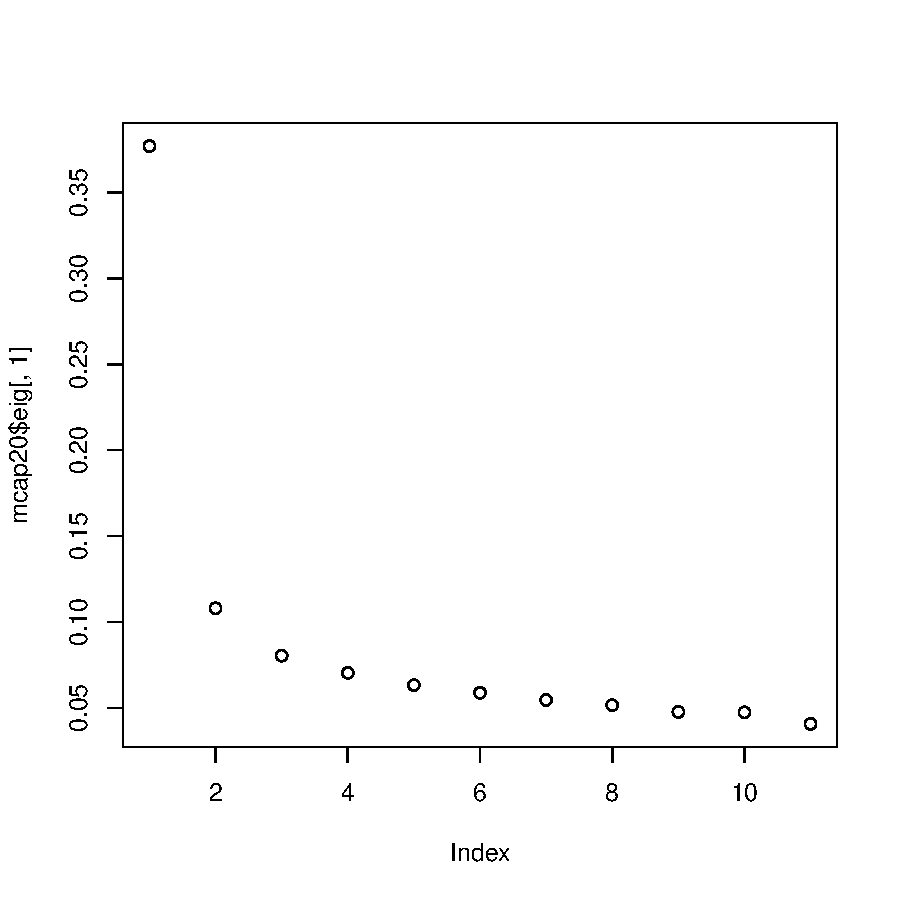
\includegraphics{6_ACM-2025-I-014}
\end{figure}
\label{fig:Vrspropios}
\end{center}
\end{frame}
% 
\begin{frame}[fragile]
\tiny
\begin{block}{R Code}
% latex table generated in R 4.5.2 by xtable 1.8-4 package
% Fri Apr 24 09:49:24 2026
\begin{table}[ht]
\centering
\begin{tabular}{rrrrrrrrrr}
  \hline
 & \begin{sideways} Coo F1 \end{sideways} & \begin{sideways} Coo F2 \end{sideways} & \begin{sideways} Coo F3 \end{sideways} & \begin{sideways} Con F1 \end{sideways} & \begin{sideways} Con F2 \end{sideways} & \begin{sideways} Con F3 \end{sideways} & \begin{sideways} Cos F1 \end{sideways} & \begin{sideways} Cos F2 \end{sideways} & \begin{sideways} Cos F3 \end{sideways} \\ 
  \hline
Si no hay castigo & 1.58 & 0.39 & 0.18 & 9.49 & 2.01 & 0.56 & 0.47 & 0.03 & 0.01 \\ 
  Si por provecho económico & 1.60 & 0.19 & 0.64 & 9.29 & 0.47 & 7.01 & 0.45 & 0.01 & 0.07 \\ 
  Si es lo acostumbrado & 1.82 & 1.09 & -0.33 & 9.29 & 11.62 & 1.45 & 0.44 & 0.16 & 0.01 \\ 
  Si alg ha hecho y ha ido bien & 1.86 & 1.17 & 0.34 & 8.37 & 11.64 & 1.32 & 0.39 & 0.15 & 0.01 \\ 
  Si pagar favor & 1.71 & 1.10 & -0.97 & 8.02 & 11.58 & 12.08 & 0.37 & 0.16 & 0.12 \\ 
  Si creencia religiosa & 1.57 & 0.20 & 1.21 & 7.36 & 0.43 & 20.43 & 0.35 & 0.01 & 0.21 \\ 
  Si resp. Ofensa honor & 1.09 & -0.30 & -0.08 & 6.96 & 1.88 & 0.16 & 0.38 & 0.03 & 0.00 \\ 
  Si alcazar objetivos & 1.11 & -0.59 & 0.32 & 6.86 & 6.81 & 2.64 & 0.37 & 0.11 & 0.03 \\ 
  Si defender prop o bienes & 0.73 & -0.21 & -0.82 & 4.76 & 1.39 & 27.69 & 0.31 & 0.03 & 0.39 \\ 
  Si lucha ley reg injusto & 0.72 & -0.63 & 0.15 & 4.67 & 12.52 & 0.93 & 0.31 & 0.24 & 0.01 \\ 
  Si ayudar familia & 0.62 & -0.60 & -0.16 & 4.14 & 13.29 & 1.25 & 0.31 & 0.28 & 0.02 \\ 
  p20b\_RDL\_AF=2\_no & -0.50 & 0.48 & 0.13 & 3.30 & 10.60 & 1.00 & 0.31 & 0.28 & 0.02 \\ 
  p20c\_RDL\_RI=2\_no & -0.43 & 0.38 & -0.09 & 2.78 & 7.47 & 0.56 & 0.31 & 0.24 & 0.01 \\ 
  p20k\_RDL\_DPB=2\_no & -0.42 & 0.12 & 0.47 & 2.74 & 0.80 & 15.95 & 0.31 & 0.03 & 0.39 \\ 
  p20f\_RDL\_OH=2\_no & -0.35 & 0.10 & 0.02 & 2.21 & 0.60 & 0.05 & 0.38 & 0.03 & 0.00 \\ 
  p20a\_RDL\_AO=2\_no & -0.34 & 0.18 & -0.10 & 2.08 & 2.07 & 0.80 & 0.37 & 0.11 & 0.03 \\ 
  p20g\_RDL\_NC=2\_no & -0.30 & -0.07 & -0.03 & 1.79 & 0.38 & 0.11 & 0.47 & 0.03 & 0.01 \\ 
  p20d\_RDL\_PE=2\_no & -0.28 & -0.03 & -0.11 & 1.65 & 0.08 & 1.25 & 0.45 & 0.01 & 0.07 \\ 
  p20i\_RDL\_LA=2\_no & -0.24 & -0.14 & 0.04 & 1.23 & 1.53 & 0.19 & 0.44 & 0.16 & 0.01 \\ 
  p20e\_RDL\_CR=2\_no & -0.22 & -0.03 & -0.17 & 1.04 & 0.06 & 2.90 & 0.35 & 0.01 & 0.21 \\ 
  p20j\_RDL\_PF=2\_no & -0.22 & -0.14 & 0.12 & 1.02 & 1.48 & 1.54 & 0.37 & 0.16 & 0.12 \\ 
  p20h\_RDL\_IB=2\_no & -0.21 & -0.13 & -0.04 & 0.94 & 1.30 & 0.15 & 0.39 & 0.15 & 0.01 \\ 
   \hline
\end{tabular}
\caption{Indicadores para análisis ordenados por contribución al F 1} 
\label{CoCnCs}
\end{table}\end{block}
\end{frame}

\begin{frame}{Interpretación del Factor 1}
En primer lugar se observa que sobre el factor 1, todas las respuestas ``Sí"\ tienen coordenadas positivas sobre el primer factor, mientras que las respuestas ``No"\ las tienen negativas.

Las mayores contribuciones y las que están mejor representadas son las respuests ``Si no hay castigo" y ``Si por provecho económico", aunque no son las que tienen las mayores coordenadas sobre dicho factor.

Las segundas mayores contribuciones y también las segundas mejor representadas son las respuestas ``Si es lo acostumbrado", ``Si alg ha hecho y ha ido bien" y ``Si pagar favor". 
Éstas tres respuestas tienen mayores contribuciones al factor 2, pero están muy mál representadas sobre él. Por tanto se consideran más como parte del factor 1 que del factor 2.
\end{frame}
% 
\begin{frame}{Interpretación del Factor 2}
Las mayores contribuciones son de las respuestas ``Si ayudar familia" y ``Si lucha ley reg injusto " y también son las mejor representadas. Las siguientes dos respuestas con altas contribuciones son ``Si es lo acostumbrado", ``Si alg ha hecho y ha ido bien", pero éstas están muy mal representadas sobre este factor y por eso se consideraron parte del factor 1.
\end{frame}
% 
\begin{frame}[fragile]
\setkeys{Gin}{width=0.6\textwidth} % para redefinir el tamaño de los graficos
\begin{figure}[H]
\centering
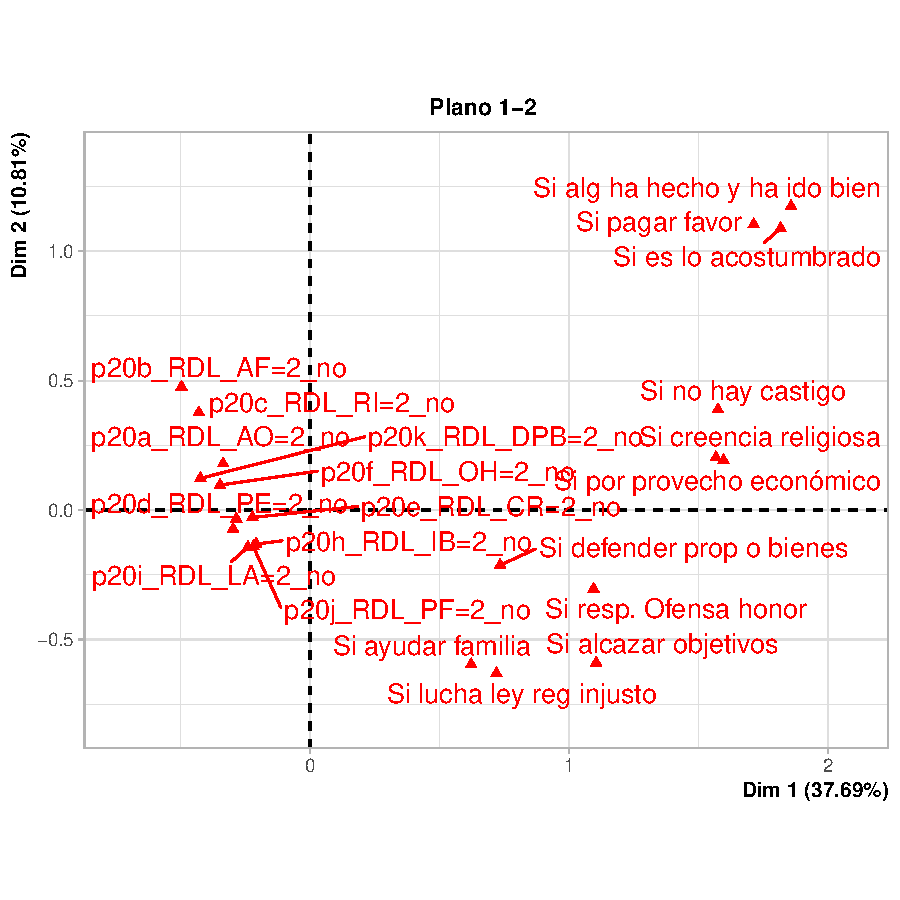
\includegraphics{6_ACM-2025-I-016}
	\caption{Plano 1-2: Sobresalen las justificaciones a la desobediencia de la ley}\label{fig:plano1-2}
\end{figure}\label{}
\end{frame}
%
\begin{frame}{Interpretación del Factor 3}
En el factor 3 predominan las altas contribuciones de las respuestas ``Si defender prop o bienes", ``Si creencia religiosa", ``No por defender prop o bienes" con coordenada negativa y ``Si pagar favor", de las cuales las tres primeras son las mejor representadas sobre dicho factor.
\end{frame}
% 
\begin{frame}[fragile]
\setkeys{Gin}{width=0.6\textwidth} % para redefinir el tamaño de los graficos
\begin{figure}[H]
\centering
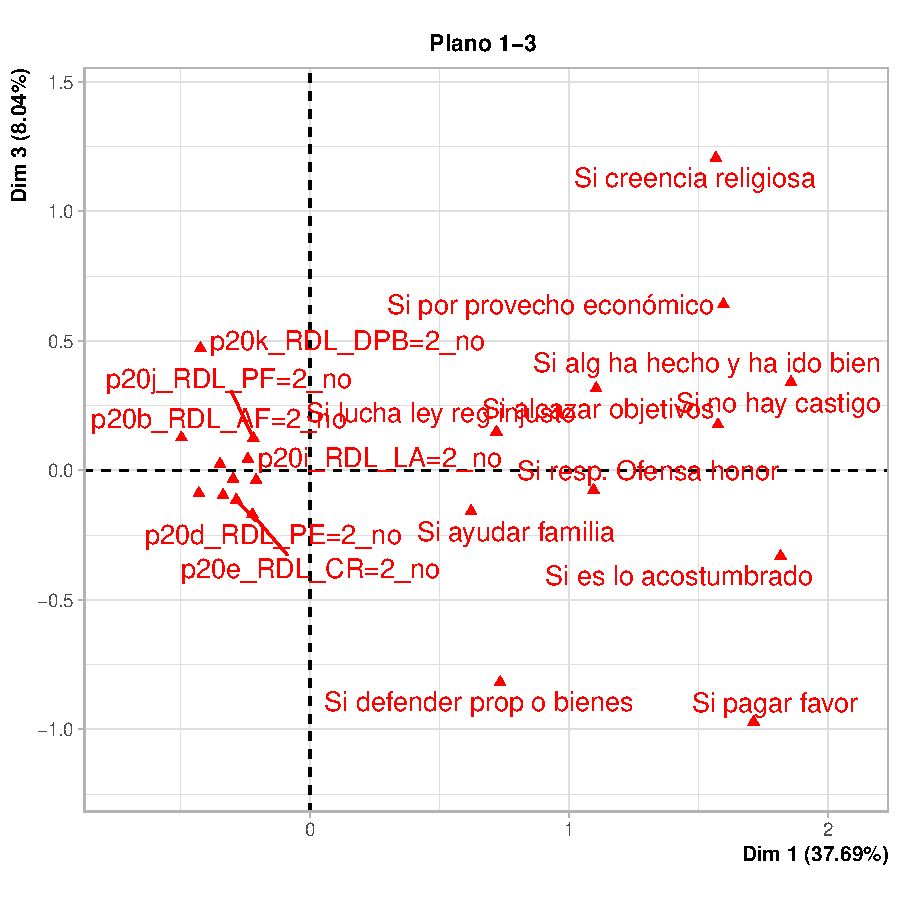
\includegraphics{6_ACM-2025-I-017}
	\caption{Plano 1-3: Sobresalen las justificaciones a la desobediencia de la ley}\label{fig:plano1-3}
\end{figure}
\end{frame}
% 
\begin{frame}[fragile]{Ejemplo: ECC-variables suplementarias}
Al incluir como suplementaria las dos preguntas acerca de la facilidad para cumplir y actuar conforme a la ley, se alcannza a observar una ligera tendencia a justificar la ley entre quienes contestaron que nunca actúan o nunca les queda fácil actuar conforme a la ley. Esta tendencia se ilustra en la gráfica \ref{fig:asocia_facl}
\end{frame}
%
\begin{frame}{Ejemplo: ECC-variables suplementarias}
\setkeys{Gin}{width=0.7\textwidth} % para redefinir el tamaño de los graficos\begin{figure}[H]
\begin{figure}
\centering
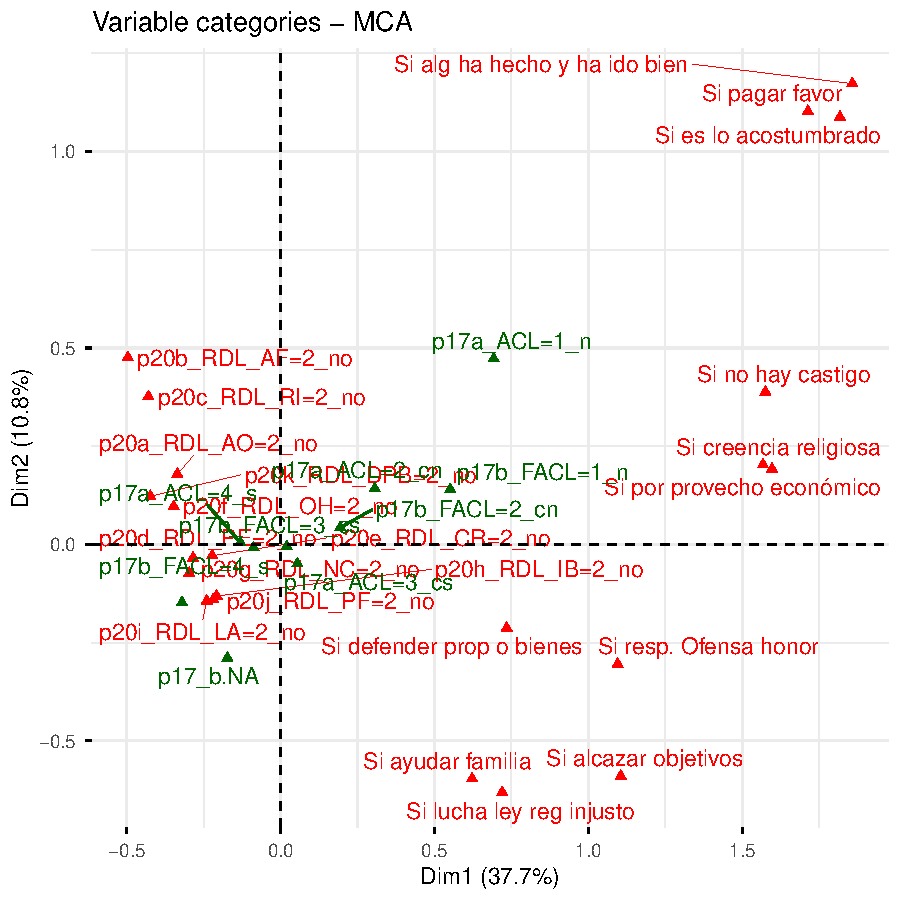
\includegraphics{6_ACM-2025-I-019}
  \caption{Asociación entre las justificaciones y la facilidad para actuar conforme a la ly}\label{fig:asocia_facl}
\end{figure}
\end{frame}
% 
\begin{frame}{fragile}
\setkeys{Gin}{width=0.6\textwidth} % para redefinir el tamaño de los graficos
\begin{figure}[H]
\centering
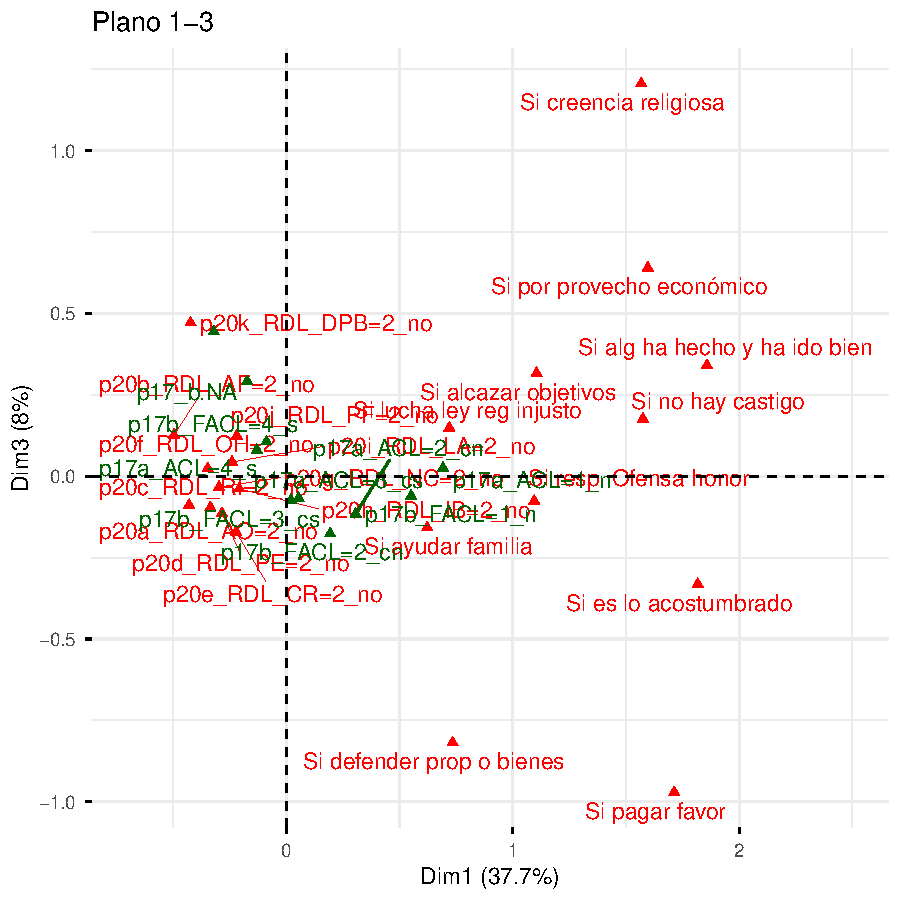
\includegraphics{6_ACM-2025-I-020}
	\caption{Plano 1-2: Sobresalen las justificaciones a la desobediencia de la ley}\label{fig:plano1-2}
\end{figure}\label{}
\end{frame}
% % 
% \begin{frame}
% 
% \end{frame}
% % 
% \begin{frame}
% 
% \end{frame}
% % 
% \begin{frame}
% 
% \end{frame}
% % 
% \begin{frame}
% 
% \end{frame}
% 
\begin{frame}{Referencias de interés}
\bibliography{BiblioMultivariado}
\end{frame}

\end{document}


